\begin{frame}
Допустимые схемы для OLAP: "снежинка", "звезда":
\begin{itemize}
\item центральным элементом являются таблицы фактов, содержащие события, транзакции, документы и др.
\item в таблице фактов одному документу (каждой его строке), соответствует одна запись.
\end{itemize}
\begin{block}{Денормализация документов в таблицу фактов}
\begin{center}
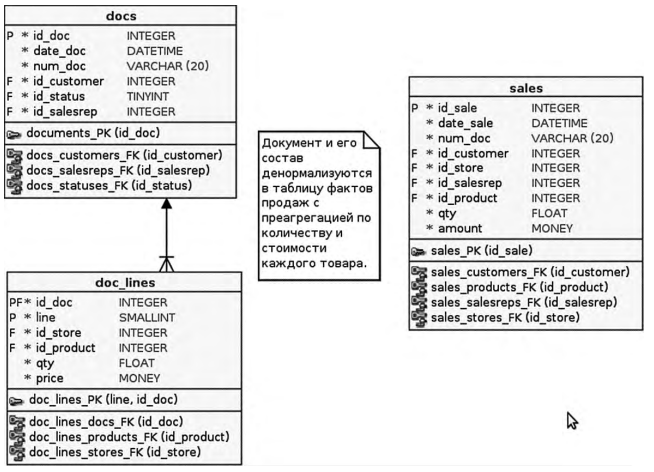
\includegraphics[scale=0.4]{images/denorm.png}
\end{center}
\end{block}
\end{frame}

\begin{frame}
\begin{block}{Пример SQL-запроса в транзакционной СУБД}
\begin{center}
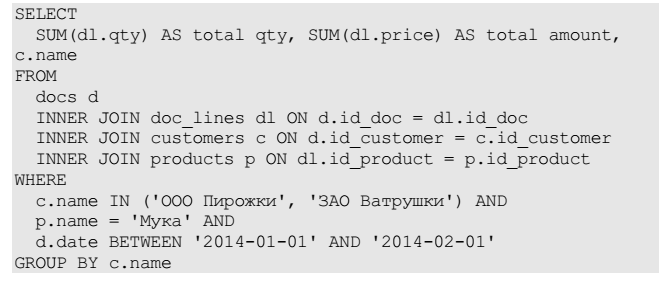
\includegraphics[scale=0.45]{images/sql-trans.png}
\end{center}
\end{block}
\begin{block}{Пример SQL-запроса в OLAP-СУБД}
\begin{center}
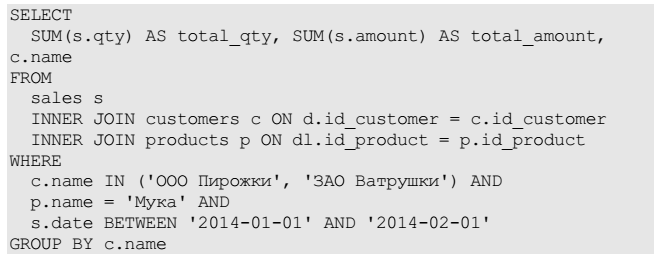
\includegraphics[scale=0.45]{images/sql-analitic.png}
\end{center}
\end{block}
\end{frame}

\begin{frame}
Если таблица фактов ссылается на таблицы-измерения, имеющие ссылки на другие измерения, то такая схема называется "снежинка".
\begin{block}{Таблица фактов в схеме "снежинка"}
\begin{center}
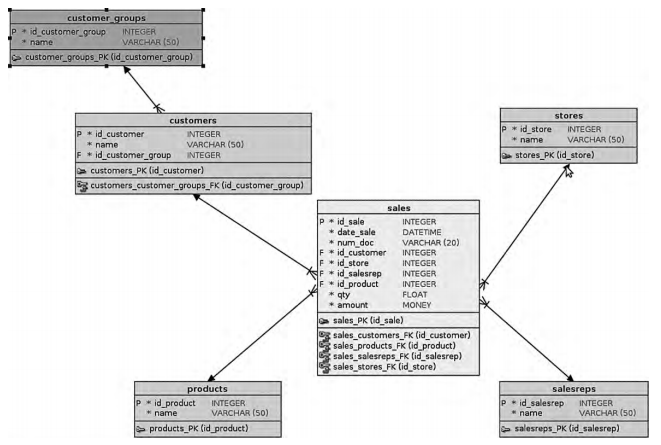
\includegraphics[scale=0.45]{images/snow.png}
\end{center}
\end{block}
Для запросов, включающих фильтрацию по группам клиентов, приходится делать дополнительное соединение.
\end{frame}

\begin{frame}
Схема "Звезда" полностью исключает иерархию измерений и необходимость соединения соответствующих таблиц в одном запросе.
\begin{block}{Таблица фактов в схеме "звезда"}
\begin{center}
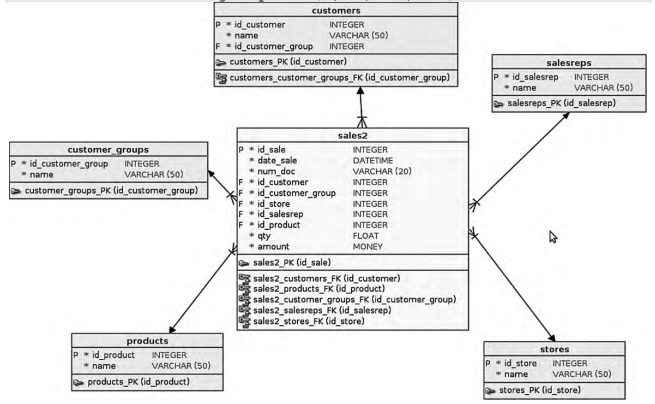
\includegraphics[scale=0.45]{images/star.png}
\end{center}
\end{block}
Обратной стороной денормализации всегда является избыточность, являющаяся причиной увеличения размера БД как в случае транзакционных, так и аналитических приложений.
\end{frame}


\begin{frame}
\begin{block}{Пример SQL-запроса в схеме "снежинка"}
\begin{center}
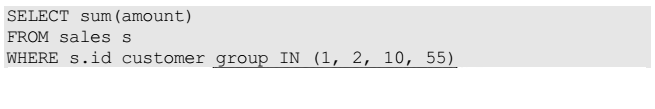
\includegraphics[scale=0.5]{images/star-sql.png}
\end{center}
\end{block}
\begin{block}{Пример SQL-запроса в схеме "звезда"}
\begin{center}
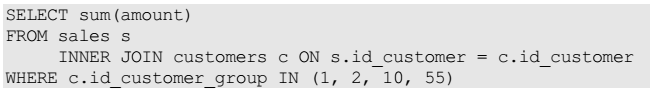
\includegraphics[scale=0.5]{images/snow-sql.png}
\end{center}
\end{block}
\begin{block}{Задача}
Посчитаем, примерную дельту на приведённом выше примере преобразования
"снежинки" в "звезду", если таблица продаж не использует компрессию данных и содержит
около 500 миллионов строк, а количество групп покупателей порядка 1000.
\end{block}
\end{frame}